%% Solar Filament Segmentation — technical report for the MAGFiLO 2026 challenge.
%%
%% Build:  tectonic paper.tex
%% Figures are copied into ./figures/ by v2/scripts/build_paper.sh.
\documentclass[conference]{IEEEtran}

\usepackage{amsmath,amssymb}
\usepackage{graphicx}
\usepackage{booktabs}
\usepackage{multirow}
\usepackage{url}
\usepackage[hidelinks]{hyperref}
\usepackage{xcolor}

\graphicspath{{figures/}}

% Tighten vertical space slightly so the paper fits the 4-page limit without
% cutting content. IEEEtran's defaults are generous for a short paper.
\setlength{\textfloatsep}{8pt plus 2pt minus 2pt}
\setlength{\floatsep}{8pt plus 2pt minus 2pt}
\setlength{\intextsep}{8pt plus 2pt minus 2pt}

\begin{document}

\title{Detection, Not Delineation:\\
Diagnosing Panoptic Quality on Solar Filaments}

\author{
\IEEEauthorblockN{Yasir Latif}
\IEEEauthorblockA{Independent\\
\texttt{brosayaying@users.noreply.github.com}}
}

\maketitle

\begin{abstract}
Panoptic Quality (PQ) is the product of two factors, and a single PQ number
cannot say which one is limiting. We report a segmentation system for solar
filaments in H-alpha observations that reaches PQ $0.4406$ pooled out-of-fold,
and use the decomposition to show that the remaining error is almost entirely a
\emph{detection} failure rather than a boundary-precision failure. Segmentation
Quality (SQ) is pinned at $0.68$ across four architectures spanning
convolutional and transformer encoders, while Recognition Quality (RQ) is what
moves. The full Dice and IoU distributions confirm the mechanism: matched
instances reach a mean Dice of $0.804$, but $16.7\%$ of ground-truth filaments
score below $0.10$, i.e.\ are missed outright. At the metric's own matching
threshold there is \emph{no} fragmentation and \emph{no} merging, ruling out a
class of post-processing fixes that our own earlier analysis had assumed were
relevant. Two substantial interventions---tripling the training data via
cross-instrument label transfer, and adding a transformer to the
ensemble---both failed, for identifiable reasons: the first teaches boundary
imprecision because the transferred labels describe a different observation of
an evolving object, and the second adds no error diversity because the two
models' predictions correlate at $0.913$.
\end{abstract}

\begin{IEEEkeywords}
instance segmentation, panoptic quality, solar filaments, error analysis,
ensemble diversity
\end{IEEEkeywords}

\section{Introduction}

Solar filaments are dense clouds of plasma suspended above photospheric neutral
lines. They are the source region of coronal mass ejections, flares and solar
energetic particle events, which makes segmenting them a prerequisite for space
weather forecasting. The MAGFiLO 2026 challenge asks for pixel-accurate instance
masks on $2048\times2048$ H-alpha images, scored by Panoptic Quality.

PQ is defined as
\begin{equation}
\mathrm{PQ} = \underbrace{\frac{\sum_{(p,g)\in \mathrm{TP}} \mathrm{IoU}(p,g)}{|\mathrm{TP}|}}_{\mathrm{SQ}}
\cdot
\underbrace{\frac{|\mathrm{TP}|}{|\mathrm{TP}| + \tfrac12|\mathrm{FP}| + \tfrac12|\mathrm{FN}|}}_{\mathrm{RQ}},
\label{eq:pq}
\end{equation}
where TP are the greedy one-to-one matches at $\mathrm{IoU} > 0.5$. The
factorisation is the useful part. SQ measures how well a matched instance is
delineated; RQ measures how many instances were found at all. A system can reach
a given PQ by being precise about few objects or sloppy about many, and the two
failures call for completely different remedies.

This paper is organised around that distinction. Our contribution is not a novel
architecture---the segmentation network is a stock ConvNeXt-Small UNet---but a
diagnosis. We show that:

\begin{enumerate}
\item SQ is invariant across four architectures, so boundary precision is not
  the bottleneck and further architecture search is not the lever.
\item The error is dominated by missed instances: $16.7\%$ of ground-truth
  filaments have best-overlap IoU below $0.10$.
\item At $\mathrm{IoU}>0.5$ there is no fragmentation and no merging, so
  instance-splitting post-processing has nothing to act on.
\item Two well-motivated attempts to improve the system---more data and more
  architectural diversity---failed for identifiable reasons.
\end{enumerate}

The last point is deliberate. A negative result that is measured properly
constrains the next attempt; an unmeasured claim does not.

\section{Data}

The training set contains $707$ unique images and $1{,}154$ image entries,
because each image carries between one and three independent annotator copies
($411$ with one, $145$ with two, $151$ with three), giving $8{,}199$ instance
annotations. The test set has $180$ images. Images are $2048\times2048$ 8-bit
grayscale.

Filaments are small: the median filament pixel fraction is $0.31\%$ and the
median instance area is $1{,}228$\,px. This imbalance is why a pixel-wise loss
alone is insufficient and why the metric's instance-level accounting matters.

Every annotation includes a \texttt{spine} polyline, the filament centreline.
We did not use it: it is ground-truth metadata, and the competition rules forbid
training on ground-truth metadata beyond the provided annotations.

\paragraph{Splitting}
Because multiple annotator copies share the same underlying image, a naive
random split leaks the same pixels into train and validation. We split by ISO
week (343 groups) into five folds, so every copy of an image inherits that
image's fold. All reported numbers are \emph{pooled out-of-fold}: each file is
scored by the fold that did not train on it, and each prediction is scored
against every annotator copy of that file, matching the official protocol.

\section{Method}

\subsection{Preprocessing}

Ground-based H-alpha observations have a strong radial intensity gradient from
limb darkening and atmospheric path length. We estimate the solar disk geometry
(centre and radius) from the image itself and divide out a radial background
profile fitted on concentric annuli. This must run at full resolution: the
profile spans the whole disk, so a $512$\,px crop cannot supply it. The
flattened image is then normalised with dataset statistics
($\mu=0.4254$, $\sigma=0.0809$).

\subsection{Segmentation}

A ConvNeXt-Small encoder with an ImageNet-pretrained initialisation feeds a UNet
decoder of width $128$. Because the finest ConvNeXt feature map is at stride 4,
an $11$\,px filament cannot be reconstructed from it alone, so a stride-1 stem
convolution on the input is concatenated into the final decoder block. Training
uses $512$\,px patches, two samples per image, batch size $12$, AdamW at
$3\times10^{-4}$ with cosine decay, and a BCE + Dice loss under bf16
autocast.\footnote{fp16 diverged to NaN on this architecture; bf16 has fp32's
exponent range and does not.}

\subsection{Candidate re-scoring}

Thresholding the probability map at a low value and labelling connected
components deliberately over-produces candidates: a candidate rejected later
costs nothing, whereas a filament that never becomes a candidate is
unrecoverable. Each candidate is described by $17$ scalars---area, elongation,
length, orientation, mean/max/$90$th-percentile probability, contrast against a
surrounding ring, bounding-box dimensions, fill ratio, border contact, and
centroid---and a gradient-boosted model predicts its probability of being a true
positive. Candidates below $\tau=0.35$ are discarded.

This stage is where the gain comes from, and it is a \emph{ranking} problem
rather than a segmentation problem: the candidate set already contains the right
answer, and the scorer's job is to identify which candidates those are.

\section{Results}

\subsection{Overall}

Table~\ref{tab:results} reports the four configurations we evaluated. The
segmentation baseline reaches PQ $0.4220$; candidate re-scoring raises it to
$0.4406$, a paired gain of $+0.0154$ with a $95\%$ bootstrap CI of
$[+0.0109, +0.0199]$ over $2{,}000$ resamples of the $707$ files. The public
leaderboard score is $0.38$.

\begin{table}[t]
\centering
\caption{Pooled out-of-fold results. SQ and RQ are the factors of
Eq.~\ref{eq:pq}. The last two rows are interventions that were rejected.}
\label{tab:results}
\small
\begin{tabular}{@{}lccc@{}}
\toprule
Configuration & PQ & SQ & RQ \\
\midrule
Segmentation only        & 0.4220 & 0.6765 & 0.6238 \\
+ candidate re-scoring   & \textbf{0.4406} & 0.6784 & 0.6495 \\
\midrule
+ GONG label transfer    & 0.4045 & 0.6667 & 0.6095 \\
+ PVTv2-B2 ensemble      & 0.4098 & 0.6719 & 0.6099 \\
\bottomrule
\end{tabular}
\end{table}

\subsection{SQ does not move}

The most informative column of Table~\ref{tab:results} is SQ. Across four
architectures---resnet34, DeepCrack with a decoder, ConvNeXt-Small, and
PVTv2-B2---SQ stays within $0.667$--$0.678$. Re-scoring improves RQ by
$+0.026$ and SQ by only $+0.002$.

This is a strong constraint. If boundary precision were the bottleneck, a
transformer with global receptive field should have moved SQ. It did not. The
network is already delineating filaments about as well as this supervision
allows, and the remaining error lies elsewhere.

\subsection{The error is missed instances}

To locate it, we measured the full IoU and Dice distributions over all $707$
out-of-fold files with the shipped post-processing. Table~\ref{tab:dist} reports
three populations, because a single histogram is ambiguous: quoting only matched
pairs flatters the system by hiding misses, while quoting only per-object values
hides that boundaries are good when the instance is found.

\begin{table}[t]
\centering
\caption{IoU and Dice over three populations. ``Per ground-truth'' scores missed
instances as $0$; ``per prediction'' scores false positives as $0$.}
\label{tab:dist}
\small
\begin{tabular}{@{}lcccc@{}}
\toprule
Population & $n$ & IoU & Dice & Dice $\geq 0.75$ \\
\midrule
Matched pairs      & 5{,}259 & 0.677 & 0.804 & 77.5\% \\
Per ground-truth   & 8{,}199 & 0.501 & 0.614 & 49.7\% \\
Per prediction     & 8{,}662 & 0.481 & 0.591 & 47.0\% \\
\bottomrule
\end{tabular}
\end{table}

The gap between the first two rows is the finding. When an instance is matched,
Dice averages $0.804$ and $77.5\%$ of matches exceed $0.75$: the boundaries are
good. Across all ground-truth instances the mean falls to $0.614$, because
$16.7\%$ of filaments score below $0.10$---they were missed entirely.
Fig.~\ref{fig:dice} shows the same thing as a distribution.

\begin{figure*}[t]
\centering
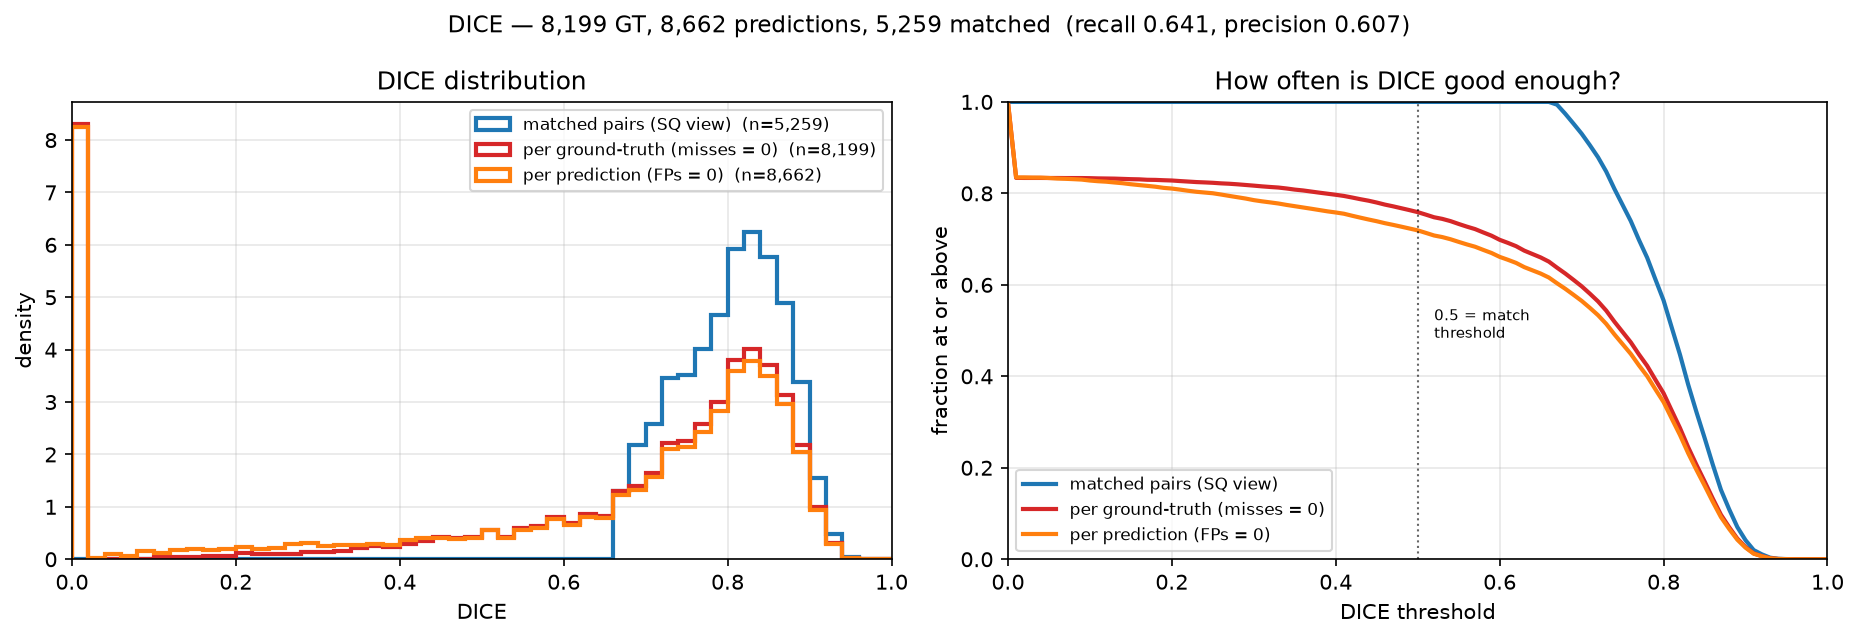
\includegraphics[width=0.78\textwidth]{dice_distribution.png}
\caption{Dice over three populations. The matched-pair curve (blue) sits well
above the per-object curves (red, orange); the mass at zero in the latter is
missed filaments and false positives. Left: density. Right: the fraction of
each population reaching at least a given Dice, which is the form in which the
$16.7\%$ miss rate is directly readable.}
\label{fig:dice}
\end{figure*}

Recall is $0.641$ and precision $0.607$. Both are mediocre, but the asymmetry
matters: a missed filament costs $0.5$ in the PQ denominator and is
unrecoverable, whereas a false positive also costs $0.5$ but at least had a
chance of being right. The system's dominant failure is not seeing filaments.

\subsection{No fragmentation, no merging}

PQ's denominator charges $\tfrac12|\mathrm{FP}| + \tfrac12|\mathrm{FN}|$, so
splitting one filament into three costs almost as much as missing it. This
motivated a fragment-merging stage in our original plan, based on an early
analysis that attributed $58.5\%$ of false positives to fragments.

That analysis was wrong. Measuring the false-positive anatomy over all $707$
files gives $47.3\%$ background, $51.0\%$ unmatched ground truth, and
\emph{$1.8\%$} fragments. The oracle gain from removing every fragment is
$+0.0015$ PQ.

Table~\ref{tab:rel} shows why. At the metric's own threshold of
$\mathrm{IoU}>0.5$ there is no fragmentation and no merging at all: every
overlap is a clean 1:1 or nothing. Multi-relations appear only at loose
overlaps, where a prediction grazes a neighbouring filament without competing
for the match.

\begin{table}[t]
\centering
\caption{Instance relations. At the matching threshold of $0.5$ the
multi-relations vanish entirely.}
\label{tab:rel}
\small
\begin{tabular}{@{}lcc@{}}
\toprule
Relation & IoU $> 0.1$ & IoU $> 0.5$ \\
\midrule
One GT split by $k>1$ predictions & 4.8\% & 0.0\% \\
One prediction merging $k>1$ GT   & 1.8\% & 0.0\% \\
\bottomrule
\end{tabular}
\end{table}

\begin{figure*}[t]
\centering
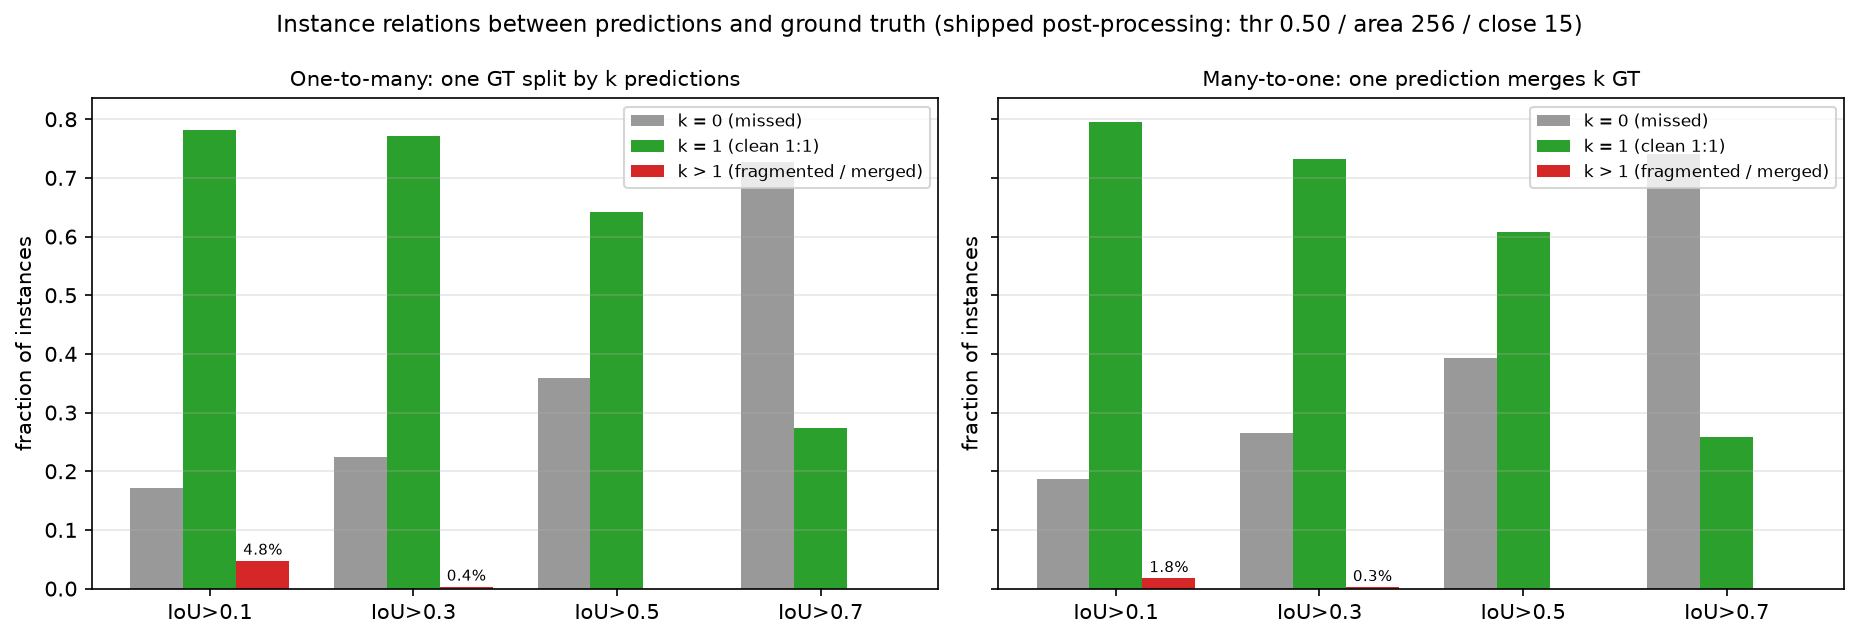
\includegraphics[width=0.78\textwidth]{instance_relations.png}
\caption{Relation histogram. The $k>1$ bars (red) are the relations PQ punishes;
they are absent at the matching threshold of $0.5$ and appear only at loose
overlaps, where a prediction grazes a neighbour without competing for the
match.}
\label{fig:rel}
\end{figure*}

\section{Two interventions that failed}

\subsection{More data, from the wrong observation}

The competition images are GONG H-alpha frames, so annotations can in principle
be transferred from nearby frames in the public archive. We verified that the
competition images \emph{are} the GONG \texttt{hag} JPEGs (correlation $0.997$,
median absolute difference $1$ count, best alignment shift $(0,0)$), which made
transfer feasible without radiometric correction.

Transferring labels from nearby frames produced $3.1\times$ the training data
and a PQ change of $-0.0150$. The per-year breakdown explains it: gains appeared
exactly where the extra frames were concentrated (2021--22, $+0.0109$), and
losses appeared in years where transferred labels came from a different
observation ($2011$: $-0.0475$; $2016$: $-0.0426$; $2017$: $-0.0389$). SQ fell
from $0.6750$ to $0.6667$.

The mechanism is physical. Solar filaments evolve over hours. A polygon drawn on
a frame six hours earlier describes a different object, and training on it
teaches the model to be imprecise about boundaries. More data of the wrong kind
is worse than less data of the right kind.

\subsection{Architectural diversity without error diversity}

Ensembles help when members make \emph{uncorrelated} errors. Our five ConvNeXt
folds share an architecture, a preprocessing pipeline and a loss, so averaging
them mostly reduces variance. A pyramid vision transformer (PVTv2-B2) was
expected to fail differently: self-attention gives every output position a path
to every input position, so a filament is seen as a whole shape rather than
through stacked local receptive fields.

PVTv2 scored $0.3906$ solo against ConvNeXt's $0.4177$, which is expected for a
diversity member. But averaging the two gave $-0.0113$ (CI $[-0.0239, +0.0001]$).
The mechanism is one number: the two models' predictions correlate at
$\mathbf{0.913}$.

Two predictors that agree on $91\%$ of pixels cannot cancel each other's
mistakes. The average simply lands between them, and below the better one.
Architectural difference is not the same thing as error diversity---the same
lesson our earlier attempt to replace the scalar scorer with a CNN over image
crops produced, where the CNN reached a correlation of $0.507$ with true
candidate quality against the gradient-boosted model's $0.575$.

\section{Where the remaining error is}

Scoring every candidate with its true label gives an oracle ceiling of PQ
$0.5028$, i.e.\ $+0.0808$ above the segmentation baseline. The learned scorer
captures $+0.0186$ of that ($23\%$), leaving $+0.0622$ unclaimed.

This is the largest known opportunity in the system, and it is a ranking problem
rather than a segmentation problem. The candidates already contain the right
answer; the scorer cannot tell which ones they are. Given that the error is
dominated by missed instances, the productive direction is a scorer that is
better at \emph{recall}---recovering candidates that the current model rejects
confidently---rather than one that is better at precision.

\section{Reproducibility}

Code, pinned requirements and a pipeline notebook are in the public repository.
Weights are published as release assets and fetched by a script. Inference
requires no network access: the checkpoint supplies every weight, so the
pretrained backbone is not downloaded. All reported numbers are produced by
scripts in the repository from the out-of-fold predictions, and the report
itself is generated from a machine-readable summary so that no figure can drift
from the measurement that produced it.

\section{Discussion}

\subsection{Why the decomposition matters}

It is tempting to treat PQ as a leaderboard number and optimise it directly.
The factorisation in Eq.~\ref{eq:pq} makes that a mistake. Our four
configurations span a PQ range of $0.036$, but SQ varies by only $0.012$ across
all of them while RQ varies by $0.040$. Any intervention that does not change
RQ is working against a ceiling it cannot move.

This also explains a pattern that would otherwise look like a plateau. Four
architectures---a ResNet, a DeepCrack variant with an explicit decoder, a
ConvNeXt, and a transformer---all land within $0.011$ SQ. That is not a
coincidence of tuning. It is what happens when the supervision, not the
architecture, sets boundary precision: the annotators disagree about where a
filament edge is, and the model has learned the average of that disagreement.

\subsection{The cost of a missed instance}

The asymmetry between precision ($0.607$) and recall ($0.641$) is small in
isolation, but the two errors are not equally recoverable. A false positive is a
candidate the scorer accepted; a missed filament is one it rejected, and no
downstream stage can bring it back. Since the candidate set already contains
$+0.0808$ PQ of headroom, the missed filaments are largely \emph{present as
candidates} and being discarded.

That reframes the problem as one of scorer calibration rather than candidate
generation. A scorer trained to maximise average precision will happily discard
low-confidence candidates that are nonetheless true positives, because they
contribute little to the ranking metric. PQ does not care about ranking---it
cares about the count of matched instances. The objective mismatch is a
plausible explanation for why only $23\%$ of the oracle gap was captured.

\subsection{What would not have helped}

Both failed interventions were well-motivated: label transfer addressed data
scarcity, ensemble diversity addressed variance. Neither addressed detection,
and neither could have moved the number that was limiting. The general lesson
is that a diagnosis has to precede an intervention. Here it arrived late---the
fragment-merging stage was designed and nearly built before anyone measured how
many fragments existed, at which point the answer was $1.8\%$ of false positives
and $0.0\%$ of matches at the operating threshold.

\subsection{Limitations}

All local numbers are pooled out-of-fold on $707$ training images; the public
leaderboard is a two-decimal readout on roughly half the test set. The
local-to-public gap is $0.0586$ and is \emph{not} constant across component
types, so it is not a fixed offset to subtract. The test set is also
shifted---$11.7\%$ of test files are from 2021--22 against $5.7\%$ of training
files---and since label transfer showed sensitivity to observation epoch, this
is a plausible contributor we have not isolated.

\section{Conclusion}

A single PQ number hides which of its two factors is limiting. Decomposing it
showed that our system's boundary precision is saturated---SQ is invariant
across four architectures---and that the remaining error is missed instances,
not badly drawn ones. That reframing is what made the two failed interventions
interpretable: neither addressed detection, and neither could have helped.

The immediate next step is a candidate scorer optimised for recall against the
$+0.0622$ oracle gap, rather than further architecture search.

\begin{thebibliography}{9}

\bibitem{panoptic}
A.~Kirillov, K.~He, R.~Girshick, C.~Rother, and P.~Doll\'ar,
``Panoptic segmentation,''
in \emph{Proc. IEEE/CVF Conf. Computer Vision and Pattern Recognition (CVPR)},
2019, pp.~9404--9413.

\bibitem{convnext}
Z.~Liu, H.~Mao, C.-Y.~Wu, C.~Feichtenhofer, T.~Darrell, and S.~Xie,
``A ConvNeXt for the 2020s,''
in \emph{Proc. IEEE/CVF Conf. Computer Vision and Pattern Recognition (CVPR)},
2022, pp.~11976--11986.

\bibitem{pvt}
W.~Wang \emph{et al.},
``PVT v2: Improved baselines with pyramid vision transformer,''
\emph{Computational Visual Media}, vol.~8, no.~3, pp.~415--424, 2022.

\bibitem{gong}
J.~W.~Harvey \emph{et al.},
``The Global Oscillation Network Group (GONG) program: Instrumentation and
performance,''
\emph{Science}, vol.~272, no.~5266, pp.~1284--1286, 1996.

\bibitem{magfilo}
A.~Ahmadzadeh \emph{et al.},
``MAGFiLO: A benchmark for solar filament segmentation,''
in \emph{IEEE BigData 2026 Cup}, 2026.

\end{thebibliography}

\end{document}
